% !TEX root = ../../../report.tex

\subsection{Software Architecture}

All the software used in the project is based on the CMSIS \cite{cmsisapi} code
base from ARM. The Giant Gecko MCU is supplied with a peripheral API, called
emlib \cite{emlibapi} which builds upon CMSIS and can be used to initialize and
control all attached peripherals. The project code and programming model is
based on the structure in emlib, see Figure \ref{fig:software-stack}.

\begin{figure}[H]
    \centering
    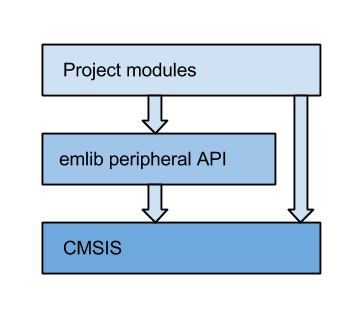
\includegraphics[height=150px]{figures/sw/software-stack.png}
    \caption{The software stack used on the microcontroller}
    \label{fig:software-stack}
\end{figure}


The application code is structured into directories representing each of the
modules, or peripherals, which have custom software written for it. Each module
contains three directories, \textit{inc}, \textit{src} and \textit{demo}.
These directories contains header files, source files, and different demos and
test programs for the modules. Each module is typically implemented as a
combination of a driver and a controller, for the peripheral it is designed for.

The custom library for Bitless includes code for setting up and controlling
all the peripherals described in the following sections.
